\chapter{Radio Telescopes}

\section{Reflectors, Antennas and Feeds}

Radio telescopes are sophisticated instruments designed to detect and analyze radio waves from astronomical sources. The core components of a radio telescope include the reflector, the antenna, and the feed. These elements work together to capture, focus, and convert radio frequency signals into a form that can be analyzed by astronomers. This section delves into the specifics of these components and their roles in the functionality of radio telescopes.

\subsection{Reflectors}

The reflector is a crucial part of a radio telescope, serving the purpose of collecting and focusing incoming radio waves onto the antenna. The most common type of reflector used in radio telescopes is the parabolic reflector. This shape ensures that radio waves parallel to the axis of the dish are reflected to a single focal point. The main features of parabolic reflectors include:

\begin{itemize}
    \item \textbf{Shape:} A paraboloid of revolution, ensuring that all incoming parallel rays are focused at the focal point.
    \item \textbf{Surface Accuracy:} The precision of the reflector surface must be within a fraction of the wavelength of the observed radio waves to avoid significant signal loss.
    \item \textbf{Size:} Reflector sizes vary, with larger dishes collecting more signal and thus allowing for the detection of weaker sources.
\end{itemize}

\subsection{Antennas}

The antenna in a radio telescope system is responsible for receiving the radio waves focused by the reflector. Several types of antennas can be used, each with its unique characteristics:

\begin{itemize}
    \item \textbf{Dipole Antennas:} Simple and effective for a range of frequencies, often used in conjunction with other elements to form more complex arrays.
    \item \textbf{Horn Antennas:} Common in microwave frequencies, providing a directional response and often used in combination with parabolic reflectors.
    \item \textbf{Array Antennas:} Consist of multiple antenna elements arranged to work together, increasing sensitivity and resolution.
\end{itemize}

Antennas convert the focused radio waves into electrical signals that can then be processed and analyzed.

\subsection{Feeds}

The feed is the interface between the reflector and the antenna. It collects the focused radio waves from the reflector and directs them to the antenna. There are different types of feeds used in radio telescopes:

\begin{itemize}
    \item \textbf{Prime Focus Feed:} Positioned at the focal point of the reflector, it directly collects the focused radio waves.
    \item \textbf{Cassegrain Feed:} Uses a secondary reflector to redirect the radio waves to a focus near the primary reflector's vertex, often allowing for more convenient placement of the receiving equipment.
    \item \textbf{Gregorian Feed:} Similar to the Cassegrain but with a concave secondary reflector, used to correct certain optical aberrations.
\end{itemize}

The choice of feed depends on factors such as the desired frequency range, the size of the reflector, and the specific scientific goals of the telescope.

In conclusion, the efficiency and effectiveness of a radio telescope depend on the precise interplay between its reflectors, antennas, and feeds. Each component must be carefully designed and optimized to ensure the maximum capture and accurate conversion of radio frequency signals from distant astronomical sources. 

\section{Heterodyne Receivers}

The purposes of the radio telescope receiver are to define the frequency range, or passband, over which the received power will be collected, and to produce a signal proportional to the collected power that can be recorded. The components that make up a receiver are often divided between two separate sections referred to as the front-end receiver and the back-end receiver.

\begin{figure}[H]
    \centering
    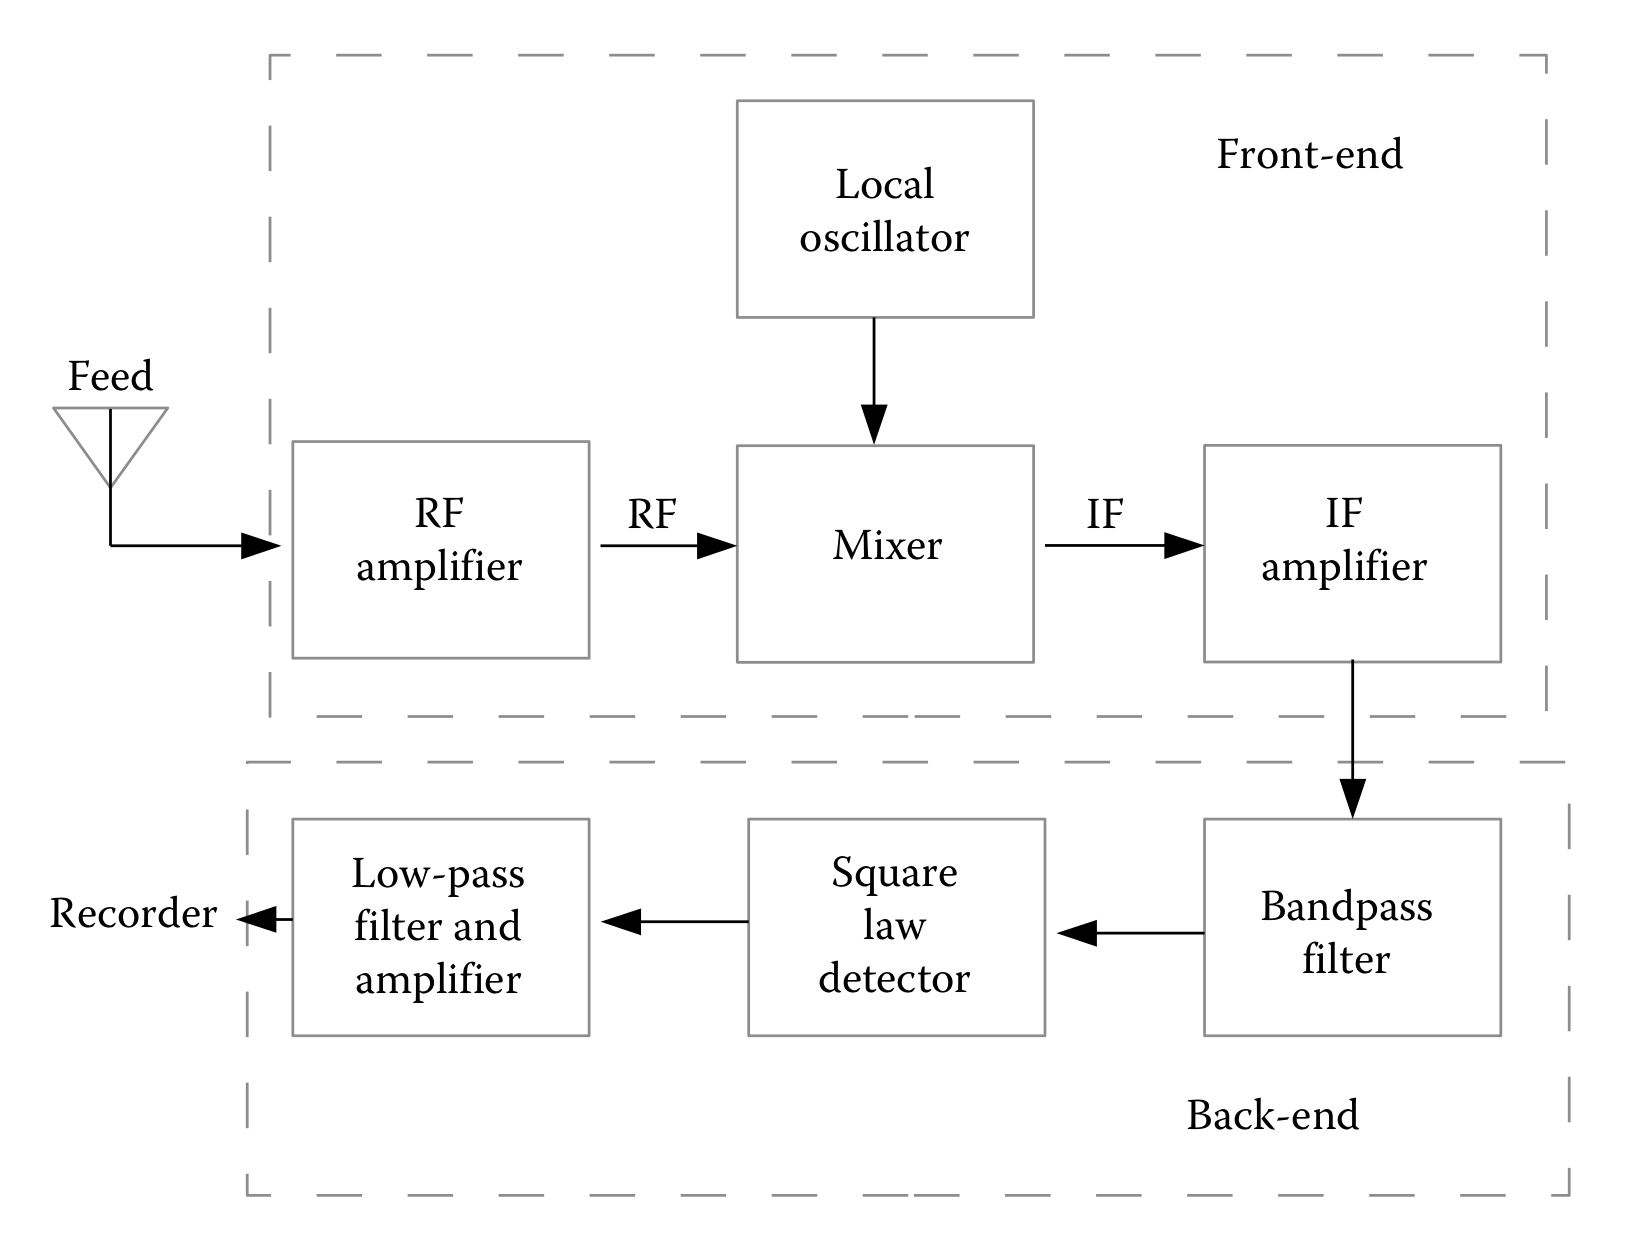
\includegraphics[width=0.8\textwidth]{Images/telescope_components.png}
    \caption{Components of a radio telescope receiver.}
    \label{fig:telescope_components}
\end{figure}

\subsection{Transmission Lines}

There are several types of transmission lines, such as waveguides and coaxial cables, used in radio telescope receivers. These transmission lines carry the electromagnetic waves from the feed to the detector. Waveguides are suitable for higher frequencies, while coaxial cables are more flexible but have higher signal loss.

\begin{figure}[H]
    \centering
    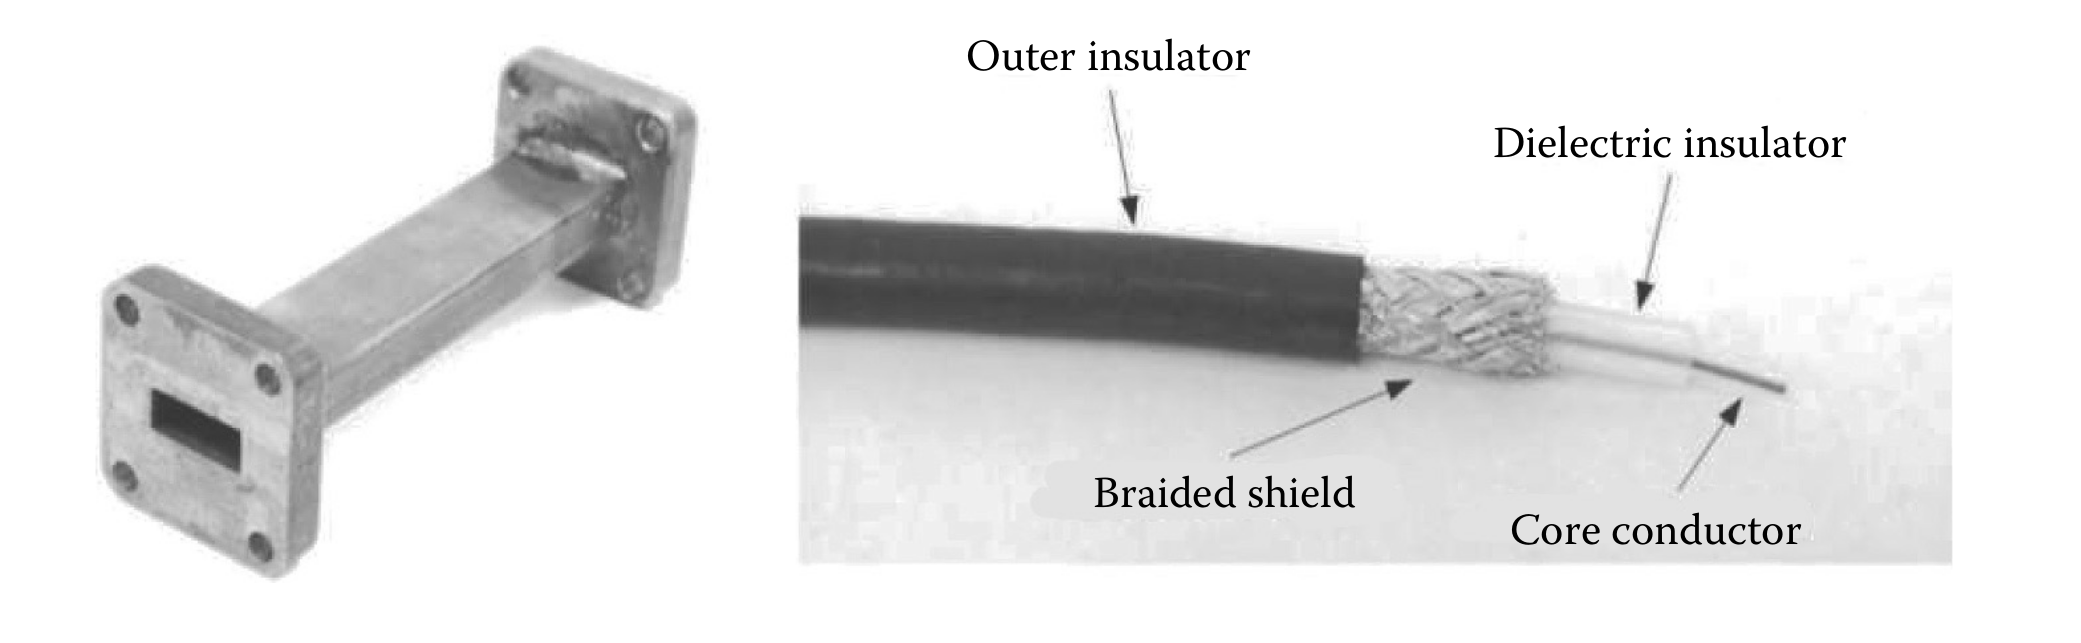
\includegraphics[width=0.8\textwidth]{Images/waveguide_coaxial.png}
    \caption{Examples of transmission lines: rectangular waveguide (left) and coaxial cable (right).}
    \label{fig:transmission_lines}
\end{figure}

\subsection{Front-End Receiver Components}

The front-end receiver components process the incoming radio frequency (RF) signals. Key components include:

\begin{itemize}
    \item \textbf{RF Amplifier:} Increases the amplitude of the RF signal.
    \item \textbf{Local Oscillator (LO):} Generates a signal used in the mixing process.
    \item \textbf{Mixer:} Combines the RF and LO signals to produce an intermediate frequency (IF) signal.
    \item \textbf{IF Amplifier:} Amplifies the IF signal for further processing.
    \item \textbf{Bandpass Filter:} Selects a narrow range of frequencies to pass to the back-end.
\end{itemize}

\subsection{Back-End Receiver Components}

The back-end receiver processes the IF signal received from the front-end. Components include:

\begin{itemize}
    \item \textbf{Bandpass Filter:} Defines the range of frequencies to detect.
    \item \textbf{Square-Law Detector:} Measures the power of the IF signal.
    \item \textbf{Low-Pass Filter:} Removes high-frequency components from the detector output.
    \item \textbf{DC Amplifier:} Amplifies the signal for digital conversion and recording.
\end{itemize}

\subsection{High-Frequency Heterodyne Receivers}

At frequencies above 300 GHz, special high-frequency heterodyne receivers are used. These receivers mix the RF signal with the IF first, then amplify the IF signal. They require low-noise components and are often based on superconducting materials.

\section{Noise, Noise Temperature, and Antenna Temperature}

Components in a receiver generate electrical signals, termed \textit{noise}, which interfere with the detection of astronomical signals. This noise is often characterized by an equivalent temperature, $T_{\text{equiv}}$, defined as:

\begin{equation}
    T_{\text{equiv}} = \frac{P}{k \Delta \nu}
\end{equation}

where $k$ is Boltzmann's constant and $\Delta \nu$ is the bandwidth. The equivalent temperature of the power delivered by the antenna is the \textit{antenna temperature}, $T_A$, while the total noise power is described by the \textit{noise temperature}, $T_N$. \\

When a signal passes through an amplifier, it is amplified by a gain factor, $G$. For a system with an amplifier of gain $G_1$ and noise temperature $T_{N1}$, the output power is:

\begin{equation}
    P = G_1 k \Delta \nu (T_A + T_{N1})
\end{equation}

For two amplifiers in succession, with gains $G_1$ and $G_2$, and noise temperatures $T_{N1}$ and $T_{N2}$ respectively, the total noise temperature is:

\begin{equation}
    T_N = T_{N1} + \frac{T_{N2}}{G_1}
\end{equation}

In general, for many components in succession:

\begin{equation}
    G = G_1 G_2 G_3 \ldots
\end{equation}

and

\begin{equation}
    T_N = T_{N1} + \frac{T_{N2}}{G_1} + \frac{T_{N3}}{G_1 G_2} + \ldots
\end{equation}

The first RF amplifier is critical in determining the total noise temperature because its gain reduces the noise contributions of subsequent components. Therefore, low-noise, high-gain RF amplifiers are crucial, and these are often cooled to near 4 K to minimize thermal noise. \\